\section{Evaluation}
	To evaluate the research and the platform that demonstrates this work, the limitations alongside future changes and additions will be discussed, ending in an evaluation of the work completed in the conclusion.
	\subsection{Limitations}

	The results regarding user time perception and information recall measurements were unexpected. While the hypothesis of heightened user engagement during interactive advertisements is not supported by the evidence gathered during the user study, the significance of the data gathered is not great enough to draw any conclusions, and further study is required. One important point to note is that the adverts in the interactive set were taken from an existing set of adverts and had overlays applied to them; that is, the adverts were not designed to be interactive. As a result, the information from the advertisement video combined with the information in the interactive overlay may have led to information overload, known to negatively impact information recall \cite{divided_attention}, as was observed in the study.

	EXPAND ON \cite{divided_attention}.
	OKAY.

	%student demographic
	% small scale
	% lmited to channel 4
	% limited to certain genres without sub genres.

	\subsection{Further work}
		\subsubsection{Programme recommendation}
		\label{sec:further_work_recommender}

		Currently, programmes are assigned binary vectors within $\mathcal{P}$; programmes either do or do not belong in each of the 18 genres. As a result, programme vectors may lie only in the corners of the hypercube geometrically representing $\mathcal{P}$. A logical improvement to the recommender system would be to allow fuzzy genre memberships, allowing programme vectors to exist anywhere within $\mathcal{P}$ and hence allowing fine-grained differences between similar programmes to be properly represented in the system.
		
		To initialize a programme with a fuzzy programme vector, \texttt{get\_programme\_vector} will be required to make use of more information than the current list of programme genres. Possible avenues to explore could include modifying $\mathcal{P}$ such that points are represented by genres pulled from multiple sources and reduced to a lower dimensionality feature space, where the feature space dimensionality would be set to minimise the number of dimensions while maximising the retained information. If additional external information processing is undesirable, user rating data could be used to modify programme vectors which are initialised as binary, although this is only useful in the case of recommending non-live programmes due to the cold start problem \citep{cold-start-problem}.

		If non-binary programme vectors are introduced to $\mathcal{P}$, a change is required in how a user vector is modified upon a negative programme rating. Under the current architecture, a user is pushed away from the vector of a negatively rated programme; if programme vectors exist away from the vertices of $\mathcal{P}$, a user who's vector somehow ends up at a vertex describing programmes they dislike will be unable to move away from the vertex by giving negative ratings, leaving them stuck. This is a difficult problem to solve and is outside the scope of this project; repeated bad ratings must not converge to a single point but explore the programme space, but must not pull a user vector away from a known `good' area. While a jump with random direction may work, storing the users previous rating will allow for exploitation of rating gradients, enabling use of more complex gradient-climbing techniques.

		The addition of implicit user ratings will remove the burden from the user of providing explicit ratings \citep{implicit_indicators}, especially if the rating interface is visually de-emphasised or removed entirely. Few interactions are offered by your4.tv from which to infer ratings from, but programme skipping is provided which carries implicit preference information \cite{exploiting_implicit_feedback}. \citep{recommender-systems-handbook}[p.~304] describe an implicit programme rating $\hat{r}$ calculated from the time a user has watched the programme $p$ and the total programme length $L$:
		$$
			\hat{r} = 3 + 2 \frac{t - 5}{L - 5},\quad 5 \leq t \leq L
		$$
		The rating given is between 3 and 5, on a rating scale of 1-5, where play times of under 5 minutes are discarded, and a rating approaches 5 as more of the programme is watched. The implicit ratings gleaned from programme skipping may be made more reliable by asking the user why the programme was skipped; this would allow the rating calculating to consider whether the user does not like the programme, or if the skip was due to another reason (they may have already seen the programme elsewhere). Although this reintroduces the problem of breaking the users pattern of activity, it may be the case that the mental cost to answer why they pressed skip is less than that of giving a rating explicitly.

		%% I think the architecture has changed so this won't work anymore.
		% The current architecture of delivering recommendations to users can be modified to allow for much greater scalability. Currently, each user requests a recommendation and the server responds. If the userbase becomes large enough for this to become infeasable, one solution is to maintain a table of user vector cluster centroids which are updated periodically by a cronjob. Periodically, this table of centroids would be multicast out to all users, along with recommendations for each centroid. 
	\subsubsection{Advert recommendation}

	If recommendation techniques are implemented to improve advert relevance, the data already being collected on user preferences will be of great value in predicting adverts the user will enjoy/engage with. Techniques have been developed \cite{contextual_advertising} which utilize this preference information, along with demographic \cite{contextual_advertising} information, which is also collected by your4.tv. A third data source utilised by the recommender system described by \cite{contextual_advertising} is user viewing histories, which your4.tv does not currently collect, though has potential to improve not only advert recommendations, but also programme recommendations, as mentioned in Section~\ref{sec:further_work_recommender}.

	\subsubsection{Waiting time/recommendation quality trade-off}
	In the current system, programme playlists are constructed in a greedy fashion, using the following algorithm:
	\begin{algorithmic}[H]
	\State start\_timestamp $\gets$ now();
	\State playlist $\gets$ $[]$;
	\While{$($totalTime(playlist) $<$ 7200$)$ \textbf{or} $($len(playlist) $<$ 4$)$}
		\State P $\gets$ $[$all live programmes starting between startTime and startTime+300$]$;
		\If{P not empty}
			\State next\_programme $\gets$ best programme in P;
		\Else
			\State next\_programme $\gets$ best non-live programme;
		\EndIf
		\State playlist.append(next\_programme);
		\State start\_timestamp $\gets$ start\_timestamp + length(next\_programme);
	\EndWhile
	\end{algorithmic}
	This is far from optimum, as programmes with extremely high predicted ratings may start at slightly over 5 minutes after the previous programme ends, leading the programme not to be recommended. By viewing playlist-building as a problem of maximizing predicted programme ratings, minimizing gaps between programmes and prioritizing live TV, this can be seen as a nontrivial constrained optimisation problem, where the trade-off values would need to be determined empirically.

	\subsubsection{Advert detection and positioning}

	Currently, MOS records (as described in section~\ref{sec:lamp-adverts}) are used to determine the location of adverts during a programme. These are inserted in the database up to one minute and eight seconds before an advert break starts. However, these records only offer up to 1 second accuracy.

	In order to replace adverts seamlessly, this accuracy must be significantly increased and hence it is useful to consider the hardware based approach taken by Inqb8r's Project4. In digital encoding systems, GPI pulses are electrical signals often used to trigger the next stage in a sequence of precisely timed events. Such electrical signals are used in the original physical cable source of television streams. Project4 receives the planned advert break information on a server with a GPI interface, precisely 8 seconds before an ad break begins. When this pulse is received it is used to insert markers into the stream with millisecond accurate precision. These markers are then used to splice adverts into the break (using a proprietary device known as the PV1000). This can be seen in \ref{Project4EventFlow}.

	%REFERENCE \citep{SCTE104} FOR GPI

	By utilising the GPI pulse to notify the media server of ad breaks in the live stream, recording could be temporarily paused until the ad break is over. This would require high precision, and so a near-constant network latency or physical proximity of the servers to the GPI pulse device would be preferable. The resulting media files would not contain any ad breaks. As a result, advert breaks in recorded programmes would not contain any small advert fragments from the original stream.

	These recordings enable arbitary insertion of ad breaks, which could be used as a platform to introduce new research questions surrounding interactive ad breaks. It is possible that the positioning, length and amount of ad breaks affects the users consumption of the media. For example, arbitary ad break lengths may discourage users from exiting the room for a specific duration. It has been found that ad breaks positioned early in a programme are more effective \citep{jeong2011position}. Analysis could also carried out as to discover the best time during a programme to position adverts or if short but often adverts outperform long and sparse positioning. A possible implementation could allow users to choose when they want to view adverts, decrementing from a total duration of adverts they must watch during a programme.

	\citet{fleming2007optimal} established a genetic algorithm to provide a local optimum of ordering advert campaigns. It is possible that the introduction of interactivity to adverts could change the required dynamic of such an algorithm, and this could be analysed using arbitary advert insertion in combination with this and other available genetic algorithms.

	Further more, arbitary advert insertion could open up further research in how users browse broadcasts (channel hopping), and how broadcasters could maximise audience reach by inserting adverts in a manner which encourages users to stay on the current channel versus other channels. E.g. position ad breaks with maximum overlap with the most competitive channel at the time. \citet{epstein1998network} showed that the monopolistic competition of broadcasters results in such an overlap, and that part of this current strategy is to analyse other broadcasters. By developing the aforementioned user-chosen advert break positioning implementation, it would be possible to analyse new strategies and also as to if user-chosen positioning can break the equilibrium created by this monopolistic competition as described by \citeauthor{epstein1998network}.


	% This is pointless, we never had individualised streams so why are we discussing it? Especially in future work. The splicing done by project4 is completely irrelevant to this project and should not be included. The only way I can see something being pulled out of this is the points on caching might be useful in a general way in terms of the future scalability of your4.

	%Finally as mentioned in \ref{sub:StreamCost} individualised streams require falling back to unicast streams which can put significant strain on the broadcaster's servers, increasing costs and reducing economic viability. Because a user could at any time skip an advert there is a potentially infinite number of necessary multicast streams needed at which point there is no benefit to multi-casting the streams. However as mentioned in \ref{sub:StreamCost}, \citet{segmentProxyCaching} and \citet{cachedStream} it is possible to reduce the strain on the broadcaster's servers by using caching proxies to redundantly cache the adverts on many servers. This is particularly useful when the data can be segmented as noted by \citet{segmentProxyCaching}. As we are using the HLS protocol \citet{HLS} which is itself a segmenting protocol our system should benefit significantly from the use of caching proxies and the adjustment of our system to include the usage of these would result in improved economic viability and would help prevent DDOS attacks on the broadcaster's servers.

	\subsubsection{Importing user personality traits}
	VisualDNA\footnote{\footurl{http://www.visualdna.com}} is a data collection company that is able to elicitate personality attributes such as interests, lifestyle, tastes, motivations and aspirations, brand preference and purchase intent specific to individual users. VisualDNA have expressed an interest in how the project could integrate personality data in order to improve programme recommendations and increase the granularity of video advert targeting.

	\begin{figure}[H]
		\centering
		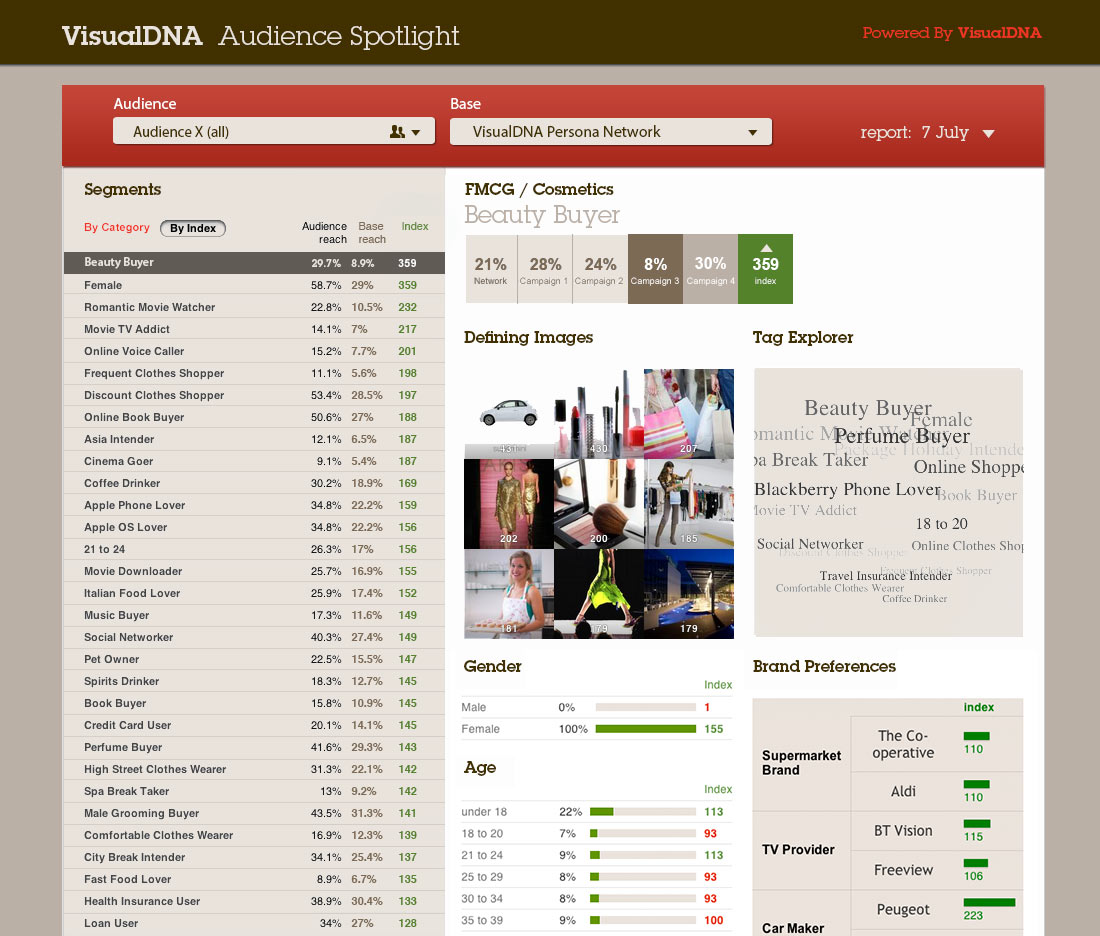
\includegraphics[width=\textwidth]{images/visualdna.jpg}
		\caption[Caption for LOF]{Visual DNA's analytics tool\footnotemark}
		\label{fig:visualdna}
	\end{figure}
	\footnotetext{\footurl{http://data.visualdna.com/audience-spotlight-advertisers}}

	Figure~\ref{fig:visualdna} shows how VisualDNA builds up psychographic profiles of users. This data is granular enough to infer information such as a users favourate supermarket or car brand. Such information is accumulated by identifying similar users and their traits, grouping them into categories, using information such as browsing history and personality quiz data. Essentially, a global recommendation engine is created which learns from this information. VisualDNA states that the usage of this information can increase advert campaign performance by ten times\footnote{\footurl{http://data.visualdna.com/targeted-advertising/}}. By using this information, advert targeting granularity could be dramatically increased.

	\citet{rentfrow2010listening} studied how personality traits affect a users preference of different genres. The paper first confirms the link between genre preference and age, ethnicity, sex, and level of education. Furthermore, the paper describes that it holds that given a constant demographics set, variances in a users personality traits produces a significant change in the genre preferences. However, \citeauthor{rentfrow2010listening} points out that the data was obtained by self-reports and so social factors may skew the results. It also points out that genres in themselves are not well-defined and often contain sub-genres which could gain a further insight. \citet{shim2007effects} also discovers the link between genres and personality traits -- e.g. it is stated that extraverts prefer reality TV shows. \citeauthor{shim2007effects}, like \citeauthor{rentfrow2010listening}, also uses a questionnaire based collection method. \citeauthor{shim2007effects} argues that the findings should not be devalued by the broad definition of genres because they are systematic categorisations based on shared characteristics. However, the paper encourages the need for future research into sub-genres.

	For these reasons, this area of research would benefit from an empirical study -- possibly by expanding the current Your4 platform to include personality data such as that provided by VisualDNA. By the active use of the system, data pertaining to the links between personality and TV genre and associated sub-genres could be collected without any undermining social factors.

\subsection{Conclusion}

In this project, we have built and tested a platform for interactive and granular targeted adverts. As part of this, we have developed a tool for content producers to deploy interactive adverts and to create targeted advertising campaigns (targeting criteria for adverts) as well as viewing the statistics pertaining to these.

We have demonstrated the use of this platform by developing a personalised TV streaming service for tablet devices, Your4, which seamlessly streams a channel to the user with programme content they most enjoy. Within this service, advertising breaks are replaced with adverts which are more likely to be of interest to the user, by taking into account their demographics and the currently playing programme. These adverts provide interactive elements, with an opportunity for creativity via the use of touchscreen gestures and controls.

The implementation stage of the project details the three major subsystems, and how these interact. This seperation of concerns, achieved with the use of REST services, a client-side application and an industry standard media server, provides a scalable and extendable platform on which to provide the Your4 service. This implementation includes a recommender subsystem to build custom playlists, which learns user preferences from user feedback, via a rating system.

Two user studies were undertaken. The first of which to determine how users consume media while watching television. The second to evaluate the use of interactive adverts on the Your4 platform. An in depth analysis of the results was documented.

% KEY PART - conclusions from studies


% I dont know what this is, but smells like bullshit
In summary our project improves the user experience by making live media personal, targeting both shows and adverts to each user as well as integrating seamlessly with the social experience. Additionally it reduces frustration at missed shows as these are transparently skipped in favour of something the user can watch from the start. In addition it provides a zero-interaction discovery system to remove the time consuming hunt for something to watch and perhaps aid users in discovering new and exciting content. Moreover it improves the experience of consuming adverts by providing users with interactivity, personally targeted adverts and the ability to control which adverts they are shown. 
